\begin{figure}[!ht] 
\label{fig:solutions/1/8/triangle_abc}
\centering
\resizebox{\columnwidth}{!}{%
%
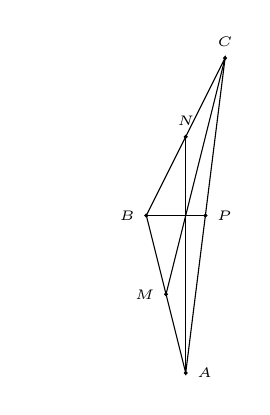
\begin{tikzpicture}
%[scale=0.5,>=stealth,point/.style={draw,circle,fill = green,inner sep=0.1pt},]
[scale=0.5,>=stealth, point/.style={draw,circle,fill = black,inner sep=0.1pt}]


%%
%%%Triangle sides
\def\a{4.12}
\def\b{4.47}
%\def\c{sqrt(\a^2+\c^2)}
\def\c{8.06}
%%
%%
%%
%%%Labeling points
%\node (A) at (0,\b)[point,label=above right:$A$] {};
%\node (B) at (\a, 0)[point,label=below left:$B$] {};
%\node (C) at (0, 0)[point,label=below right:$C$] {};
%\node (M) at (\a*0.5,\b*0.5)[point,label=above:$M$] {};
%\node (D) at (\a,\b)[point,label=above right:$D$] {};
%%
%%
%%%Drawing triangle ABC
%\draw (A) -- node[below] {$\textrm{}$} (B) -- node[left] {$\textrm{a}$} (C) -- node[above,xshift=5mm] {$\textrm{b}$} (A);
%%
%%%Joining CD
%\draw (C)--(D);
%%%Joining BD
%\draw (B)--(D);
%%
%%%Drawing and marking angles
%%\tkzMarkAngle[fill=orange!40,size=0.5cm,mark=](A,M,C)
%%\tkzMarkAngle[fill=orange!40,size=0.5cm,mark=](B,M,D)
%%\tkzMarkAngle[fill=green!40,size=0.5cm,mark=](A,B,C)
%%\tkzMarkRightAngle[fill=blue!20,size=.2](A,C,B)
%%\tkzMarkRightAngle[fill=blue!20,size=.2](D,B,C)
%%\tkzLabelAngle[pos=0.65](A,M,C){$\theta$}
%%\tkzLabelAngle[pos=0.65](B,M,D){$\theta$}
%%\tkzLabelAngle[pos=0.65](A,B,C){$\alpha$}
%%


% the coordinates of the vertices
\coordinate (A) at (4,-6);
\coordinate (B) at (3,-2);
\coordinate (C) at (5,2);


\coordinate (M) at (3.5,-4);
\coordinate (N) at (4,0);
\coordinate (P) at (4.5,-2);

% the axis
\draw[thin,scale=0,-] (-1,0) -- (5.5,0);
\draw[thin,scale=0,-] (0,-2.5) -- (0,2.5);

% the edges of the triangle
\draw (A) -- (B) -- (C) -- cycle;
\draw[-] (B) -- (P) ;
\draw[-] (A) -- (N) ;
\draw[-] (C) -- (M) ;

% labelling the vertices
%\node (A) at (4,-6)[point,label=above right:$A$] {};
\node[point,label={right:\tiny $A$}] at (A) {};
\node[point,label={left:\tiny $B$}] at (B) {};
\node[point,label={above:\tiny $C$}] at (C) {};
\node (M) at (3.5,-4)[point,label=left:\tiny $M$]{};
\node (N) at (4,0)[point,label=above:\tiny $N$] {};
\node (P) at (4.5,-2)[point,label=right:\tiny $P$] {};

% the arcs for the angles
%\begin{scope}[black]
%\draw[->]
%  (1,0) +(0:0.5cm) arc [radius=1cm,start angle=0,end angle=41] node[midway,right] {$\alpha$};
%\draw[->]
%  (0.5,0) +(0:0.25cm) arc [radius=0.75cm,start angle=0,end angle=122] node[midway,above] {$\beta$};
%\end{scope}
%
\end{tikzpicture}
%



%\begin{tikzpicture}[scale=.5]
%  \tkzDefPoint(4,-6){A} \tkzDefPoint(3,-2){B}
%  %\tkzDrawCircle[R,dashed](A,7 cm) \tkzDrawCircle[R,dashed](B,13 cm)
%  \tkzInterCC[R](A,4.12 cm)(B,4.47 cm) \tkzGetPoints{C}{D}
%  \tkzDrawPolygon(A,B,C)
%  \tkzCompasss(A,C B,C)
%  \tkzLabelSegment[below](A,B){$4.12$ cm}
%  \tkzLabelSegment[above left](A,C){$4.47$ cm}
%  \tkzLabelSegment[above right](B,C){$8.06$ cm}
%  \tkzDrawPoints[color=red](C)
%  \tkzDrawPoints[color=blue](A,B)
%\end{tikzpicture}
}
\caption{$\triangle ABC$}
\end{figure}
Given that two angles of traingle are equal,
\begin{align}
    \label{eq:solutions/1/8/1}\angle{ABC}&=\angle{ACB}\\[5pt]
\cos\angle{ABC} &= \cos\angle{ACB}\\[5pt]
    \label{eq:solutions/1/8/2}\frac{(\vec{B}-\vec{A})^T(\vec{B}-\vec{C})}{\norm{\vec{B}-\vec{A}}\norm{\vec{B}-\vec{C}}} &= \frac{(\vec{C}-\vec{A})^T(\vec{C}-\vec{B})}{\norm{\vec{C}-\vec{A}}\norm{\vec{C}-\vec{B}}}\\[7pt]
    \label{eq:solutions/1/8/3}\frac{(\vec{B}-\vec{A})^T(\vec{B}-\vec{C})}{\norm{\vec{B}-\vec{A}}} &= \frac{(\vec{C}-\vec{A})^T(\vec{C}-\vec{B})}{\norm{\vec{C}-\vec{A}}}
\end{align}
It can be showed that,
% \norm{\vec{B}}^2 - \vec{B}^T\vec{C} - \vec{A}^T\vec{B} + \vec{A}^T\vec{C}
% $\norm{\vec{B}}^2 = \norm{\vec{A}-\vec{B}}^2 - \norm{\vec{A}}^2 + 2\vec{A}^T\vec{B}$
\begin{multline}
    \label{eq:solutions/1/8/4}
(\vec{B}-\vec{A})^T(\vec{B}-\vec{C}) = \norm{\vec{A}-\vec{B}}^2 - (\vec{A}-\vec{C})^T(\vec{A}-\vec{B})
\end{multline}
\begin{multline}
    \label{eq:solutions/1/8/5}(\vec{C}-\vec{A})^T(\vec{C}-\vec{B}) = \norm{\vec{A}-\vec{C}}^2 - (\vec{A}-\vec{C})^T(\vec{A}-\vec{B})
\end{multline}
Substituting \eqref{eq:solutions/1/8/4} and \eqref{eq:solutions/1/8/5} in \eqref{eq:solutions/1/8/3},
{\footnotesize
\begin{align}
\label{eq:solutions/1/8/6}\frac{\norm{\vec{A}-\vec{B}}^2 - (\vec{A}-\vec{C})^T(\vec{A}-\vec{B})}{\norm{\vec{B}-\vec{A}}}&=\frac{\norm{\vec{A}-\vec{C}}^2 - (\vec{A}-\vec{C})^T(\vec{A}-\vec{B})}{\norm{\vec{C}-\vec{A}}}\\
\label{eq:solutions/1/8/7}\norm{\vec{A}-\vec{B}} - \frac{(\vec{A}-\vec{C})^T(\vec{A}-\vec{B})}{\norm{\vec{B}-\vec{A}}}&=\norm{\vec{A}-\vec{C}} - \frac{(\vec{A}-\vec{C})^T(\vec{A}-\vec{B})}{\norm{\vec{C}-\vec{A}}}\\
\label{eq:solutions/1/8/8}\norm{\vec{A}-\vec{B}} - \norm{\vec{A}-\vec{C}} \cos{\angle{BAC}}&=\norm{\vec{A}-\vec{C}} - \norm{\vec{A}-\vec{B}} \cos{\angle{CAB}}\\
\label{eq:solutions/1/8/9}\norm{\vec{A}-\vec{B}} +  \norm{\vec{A}-\vec{B}} \cos{\angle{CAB}}&=\norm{\vec{A}-\vec{C}} + \norm{\vec{A}-\vec{C}} \cos{\angle{BAC}}\\
\label{eq:solutions/1/8/10}\norm{\vec{A}-\vec{B}}(1 + \cos{\angle{CAB}})&=\norm{\vec{A}-\vec{C}}(1 + \cos{\angle{BAC}})\\
\implies\norm{\vec{A}-\vec{B}} &= \norm{\vec{A}-\vec{C}}
\end{align}
}
